% !TEX root = ../thesis-sample.tex

\chapter{LSPR response to Bovine Serum Albumin} \label{chap:lspr_response_bsa}
\graphicspath{{lspr_response_bsa/figs/}}

Localized surface plasmon resonance (LSPR) biosensors detect target molecules
by tracking frequency shifts in the plasmon resonance of metallic nanoparticles
in the presence of analytes \cite{WilletsVandyune2007}. The chapter presents the 
modeling of LSPR biosensors using \pygbe. We compute the extinction cross section 
of a silver nanosphere with bovine serum albumin (BSA) proteins (PDB code: 4FS5,
BSA dimmer) in different locations around it. 


{\color{red}
We might need to add something else here
}

\section{Grid convergence analysis} \label{sec:grid_conv_bsa}
We perform a grid convergence study to ensure that the meshes are correctly
resolving the numerical solutions. We performed the convergence analysis of
the system sketched in in Figure \ref{fig:analyte-sensor}. Given that we 
compute the extinction cross section by integrating over the sphere, we set 
a fixed mesh density for the protein and refined the mesh of the nanosphere 
(512, 2048, 8192, 32768 elements). For the protein, we found that a mesh with
two triangles per $\text{\AA}^2$ was fine enough for the convergence 
analysis, resulting in $N_{prot} = 98116$ elements.
We use the same conditions used in the grid convergence analysis of the 
isolated nanoparticle of section \ref{sub_sec:grid_conv_iso}, presented
in Tables \ref{table:quadparams1} and \ref{table:treeparams1}. The protein 
dielectric constant for a wavelength of 380 nm is $2.7514 + 0.2860i$, this  
value was computed using a functional relationship provided by Phan
 et al.~\cite{PhanETal2013}. The protein was located at a distance of 
 $d=$ 1 nm of the sphere along the z-axis, such that its dipole moment 
 was aligned with the y-axis. We show the errors in Figure  \ref{fig:err_sph-bsa} 
 and table \ref{table:err_sph-bsa} which were computed using the Richardson extrapolated
{\color{red} (see Section, cite section that explains rich extra)} value of 
the extinction cross section $C_{ext}= 1778.73$ nm$^2$.

\begin{figure}%[h] %  figure placement: here, top, bottom, or page
    \centering
    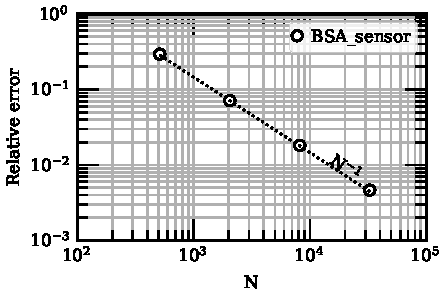
\includegraphics[width=0.65\textwidth]{convergence_bsa_sensor_R8_d1_w380.pdf} 
    \caption{Grid-convergence study of extinction cross-section of a spherical silver
             nanoparticle with a BSA protein at $d=1$ nm. 
             Figure, plotting script and auxiliary files available 
             under \textsc{cc-by} \cite{ClementiETal2018c}.}
    \label{fig:err_sph-bsa}
 \end{figure}

 \begin{table}%[h]
    \centering
    \caption{\label{table:err_sph-bsa} Estimated percentage error of the BSA-sensor 
    system (Fig.~\ref{fig:analyte-sensor}), with respect to the extrapolated value 
    (using Richardson extrapolation).} 
    \begin{tabular}{c c}
    \hline%\toprule
    N & \% error \\
    \hline%\midrule
     $512$ & $29.39$ \\
     $2048$ & $7.13$ \\
     $8192$ & $1.82$ \\
     $32768$ & $0.46$ \\
    \hline%\bottomrule
    \end{tabular}
\end{table}

The observed order of convergence is 0.99, and we can see in Figure
\ref{fig:err_sph-bsa} that the error decays with the number of boundary elements
at a rate of $1/N$, which is consistent with the verifications results showed
in Section \ref{sec:verification}. This shows that the numerical solutions computed
with \pygbe are correctly resolved by the meshes.

\section{Plasmon resonance frequency shifts} \label{sec:shift_bsa}

When a target molecule approaches the metallic nanoparticle, the resonance frequency
of this nanoparticle shifts. In this section, we computed the LSPR response as a
function of the wavelength in the presence of BSA protein. We optimized run times 
without compromising accuracy by using a relaxed set of parameters. For the protein
mesh density we used one element per $\text{\AA}^2$ ($N_{prot} = 45140$) and for the
sphere mesh we used $N_{sensor} = 32768$ elements. These calculations used the same
parameters from Tables \ref{table:quadparams2} and \ref{table:treeparams2}, which 
resulted in a percentage error below $1\%$, with respect to the Richardson-extrapolated
value. The run time for one frequency when two proteins are present, is approximately 
$15$ min using a NVIDIA Tesla K40c GPU.



\begin{center}
    \begin{figure} %  figure placement: here, top, bottom, or page
       \centering
       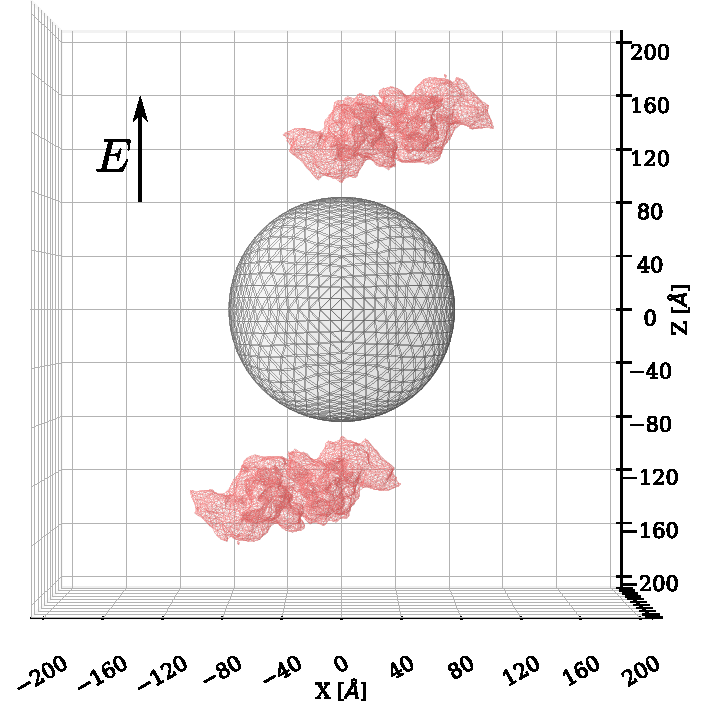
\includegraphics[width=0.65\textwidth]{2prot_1nm_z_R8nm.pdf} 
       \caption{Sensor protein display: BSA located at $\pm 1$ nm of the 
                nanoparticle in the $z$-direction. Figure, plotting script and auxiliary 
                files available under \textsc{cc-by} \cite{ClementiETal2018e}.}
       \label{fig:display_z}
    \end{figure}
    \end{center}

Figure \ref{fig:display_z} shows a visualization of the meshes setup for these 
calculations, with two BSA proteins located at $d=1$ nm away from the spherical 
silver nanoparticle, along the $z$ axis. The position of the BSA molecule at $+z$ 
axis was the same used for the convergence analysis in section \ref{sec:grid_conv_bsa},
while the protein located in the $-z$ position is a 180$^\circ$ solid rotation 
about the $y$ axis, of the BSA in $+z$.  Figure \ref{fig:2pz_response} shows the results
of the calculations between 382 and 387 nm every $0.25$ nm, near the peak seen in Figure
\ref{fig:verif_sph}. In Figure \ref{fig:2pz_response} we have the variation of the 
extinction cross section with respect to wavelength for the isolated nanoparticle 
($d=\infty$) and with BSA proteins located at $d=1$ nm apart from the nanosphere. The
result shows a redshift ($0.5$ nm) in the resonance frequency due to the presence of 
the BSA analytes.

\begin{figure} %[h] %  figure placement: here, top, bottom, or page
    \centering
    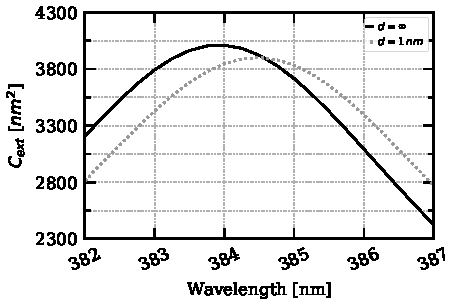
\includegraphics[width=0.65\textwidth]{2pz_R8nm.pdf} 
    \caption{Extinction cross-section as a function of wavelength for an $8$ nm
             silver sphere immersed in water with two BSA proteins placed 
             $\pm 1$ nm away from the surface in the $z$-direction, and at
             infinity (no protein).}
    \label{fig:2pz_response}
 \end{figure}

Figure \ref{fig:2pz_response} shows a redshift of the plasmon resonance frequency 
peak in the presence of two BSA proteins located at 1 nm along the $z$ axis. Experimental 
observations in the work of Tang, et al.~\cite{TangETal2010} revealed a redshift when 
BSA proteins in a solution are added to silver nanoparticles of approximately $17$ nm 
in diameter. They also observed a decrement of the peak amplitude, similarly to the 
effects we see with our model. Moreover, recent experiments \cite{PuETal2018} report 
resonance frequency between $380$ and $400$ nm for a silver nanosphere in the presence
of BSA proteins (check reference and its supplementary material), which is consistent with 
our results. Other experiments \cite{RaphaelETal2013} also report redshifts in the presence
of different proteins. The boundary element method approach that we implemented using 
electrostatic approximation is thus able to capture the characteristics of LSPR biosensors
based on resonance-frequency shift. 

We also study the effect of the location of the proteins, we performed the same 
calculations but now placing the BSA analytes along the $x$ and $y$ axis at $\pm 1$ nm,
as shown in Figure \ref{fig:display_xy}. We obtain these configurations by performing
a 90$^\circ$ solid rotation of the $z$-configuration (Figure \ref{fig:display_z})
along the $x$- and $y$-axis, respectively. Figure \ref{fig:2pxy_response} shows the 
results for each configuration.

 \begin{figure}
    \centering
    \subfloat{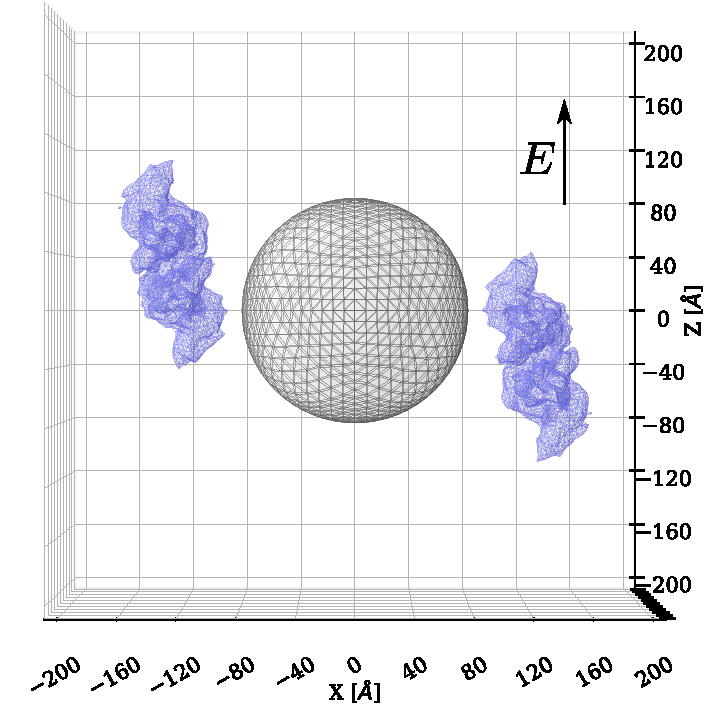
\includegraphics[width=0.65\textwidth]{2prot_1nm_x_R8nm.pdf}} \\
    \subfloat{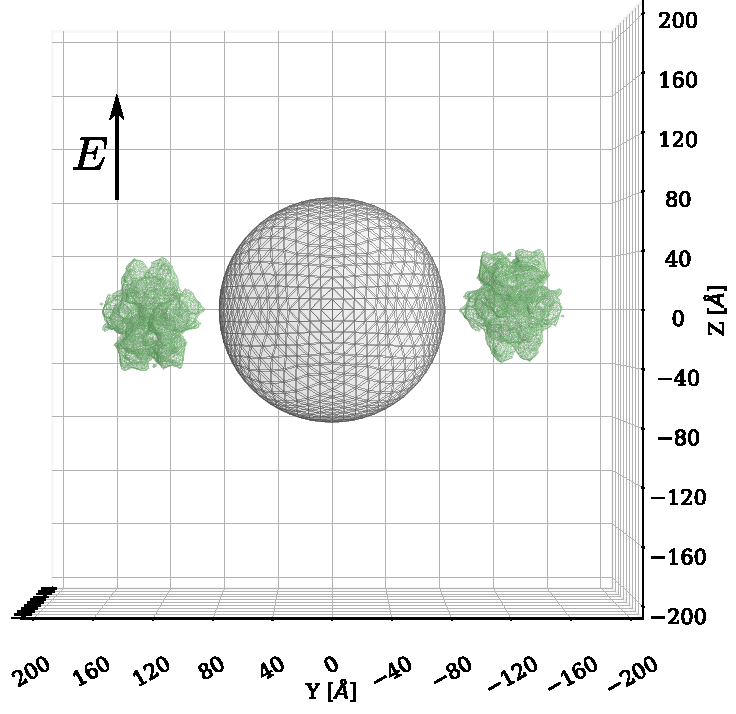
\includegraphics[width=0.65\textwidth]{2prot_1nm_y_R8nm.pdf}} 
     \caption{Sensor protein display: BSA located at $\pm 1$ nm of the nanoparticle in the
            $x$-direction (top) and $y$-direction (bottom). Figure, plotting script and 
            auxiliary files available under \textsc{cc-by} \cite{ClementiETal2018e}.}
     \label{fig:display_xy}
 \end{figure}

 \begin{figure}%[t] %  figure placement: here, top, bottom, or page
    \centering
    \subfloat{\includegraphics[width=0.65\textwidth]{{2px_R8nm}.pdf}}\\
    \subfloat{\includegraphics[width=0.65\textwidth]{{2py_R8nm}.pdf}} 
    \caption{Extinction cross-section as a function of wavelength for an $8$-nm
             silver sphere immersed in water with two BSA proteins placed at
             $\pm 1 $ nm away from the surface in the $x$-direction (top) and
             $y$-direction (bottom), and at infinity (no protein).}
    \label{fig:2pxy_response}
 \end{figure}

Figure \ref{fig:display_xy} shows the configuration where the proteins are placed at a 
distance in the $x$ (top) or $y$ (bottom) direction. For these configurations and with 
the electric field aligned with the $z$ axis, the LSPR response is negligible. The 
frequency shifts in Figure \ref{fig:2pxy_response} are smaller than the wavelength 
resolution ($<0.25$ nm). This finding is consistent with the free electrons oscillating
along the $z$ axis under a $z$-polarized electric field, and not in the $x$ and $y$ 
directions {\color{red} ADD REFERENCE TO FIG OF OSCILLATING ELECTRONS - LSPR}. The 
proteins have a marked effect when placed in the $z$ direction, where they can interfere 
with the oscillation of the free electrons. 

\section{Sensitivity study} \label{sec:sensitivity}

On LSPR biosensors we refer to sensitivity to the relationship between the size of the 
resonance frequency shift and the number of analytes bound to the sensor (through the 
ligand). Experiments show that the distance between the protein and the nanoparticle 
affects the sensitivity of the sensor, to the point that targets placed 15 nm away 
from the surface are hardly detectable \cite{HaesETal2004}. This is a critical issue
considering that most common ligands, like antibodies, can be larger than 15 nm. In 
Figure \ref{fig:dist_response} we can see how the resonance peak varies with the distance 
at which the  analytes are located ($+z$ and $-z$). When $d=2$ nm we have a shift of 
$0.25$ nm while when the analytes are at $d=0.5$ nm the shift is $0.75$ nm. The parameters
used in these simulations remain the same as the ones used for the cases in Figures 
\ref{fig:2pz_response} and \ref{fig:2pxy_response}.

\begin{figure}%[h] %  figure placement: here, top, bottom, or page
   \centering
   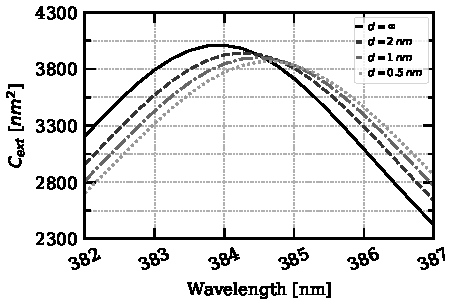
\includegraphics[width=0.65\textwidth]{2pz_lspr_response.pdf} 
   \caption{Extinction cross-section as a function of wavelength for an $8$-nm
            silver sphere immersed in water with two BSA proteins placed at
            $2$, $1$, and $0.5$ nm away from the surface in the 
            $z$-direction, and at infinity (no protein). The test case with
            $d=0.5$nm is close to the limit where quantum tunneling might happen. 
            Such effects are not captured by our classical model.}
   \label{fig:dist_response}
\end{figure}

As expected, Figure \ref{fig:dist_response} shows how the shift decreases as the BSA 
proteins move away from the nanoparticle, to the point that we only see a shift of 
$0.25$ nm when the analyte is $2$ nm away. This results shows the potential of \pygbe 
and the electrostatic approach to study biosensors sensitivity with distance. It's 
worth noting that quantum effects (e.g., tunneling) at $d=0.5$ nm are ignored with 
our classical approach. Even if this distance could be close to the quantum regime, 
there is evidence that classical theory is valid at this distance in similar systems
\cite{SavageETal2012, EstebanETal2012}

Even though there is evidence that techniques such as plasmon-enhanced Raman 
scattering are capable of detecting to the single-molecule limit 
\cite{ZhangZhangETal2013}, as far as we know there is no evidence of a purely
LSPR approach that can sense such low concentrations of proteins. Our 
computational results can unveil potential improvements that would enhance 
the sensitivity of LSPR biosensors, for example by using smaller ligands. 

There are not other LSPR simulations where the molecular details of the analyte 
are considered, that we are aware of. However, similar calculations can be 
performed with other open source softwares like BEM++ \cite{SmigajETal2015} and 
MATLAB toolbox MNPBEM \cite{HohenesterTrugler2012}. BEM++ also models the system
as a set of boundary integral equations, discretized in flat triangular panels, 
and it uses a Galerkin approach and algorithmic acceleration via hierarchical 
matrices. MNPBEM is another alternative software designed to simulate scattering
of metallic nanoparticles, which its BEM implementation is similar to \pygbe 
(centroid collocation with flat triangles) but with different acceleration scheme.
This MATLAB toolbox, similarly to BEM++, also relies on hierarchical matrices 
rather than a treecode, resulting in higher memory usage compared to our code, 
making it harder to simulate large analytes in detail. 
Commercial finite-element or finite-difference solvers can also be used for this
type of application, for example COMSOL. However, these volumetric approaches 
struggle to correctly impose the zero boundary condition at infinity, which is
exactly met for BEM.  
